
\chapter{Introducción}

La piel es considerada el órgano mas grande del cuerpo humano,  y está compuesta por tres capas: \emph{\gls{epidermis}}, \emph{\gls{dermis}} e \emph{\gls{hipodermis}} (figura \ref{fig:skin1_jpg}). La principal función de la piel es proteger al cuerpo de las hostilidades del medio ambiente como la radiación solar y los factores externos como las bacterias, sin embargo también cumple otras funciones importantes aparte de proteger los órganos y los tejidos internos, tales otras funciones son regular nuestra temperatura corporal, registrar sensaciones de presión, frío, calor y es una interfaz para poder sentir e interactuar con lo que tenemos a nuestro alrededor.

\begin{figure}[h!]
    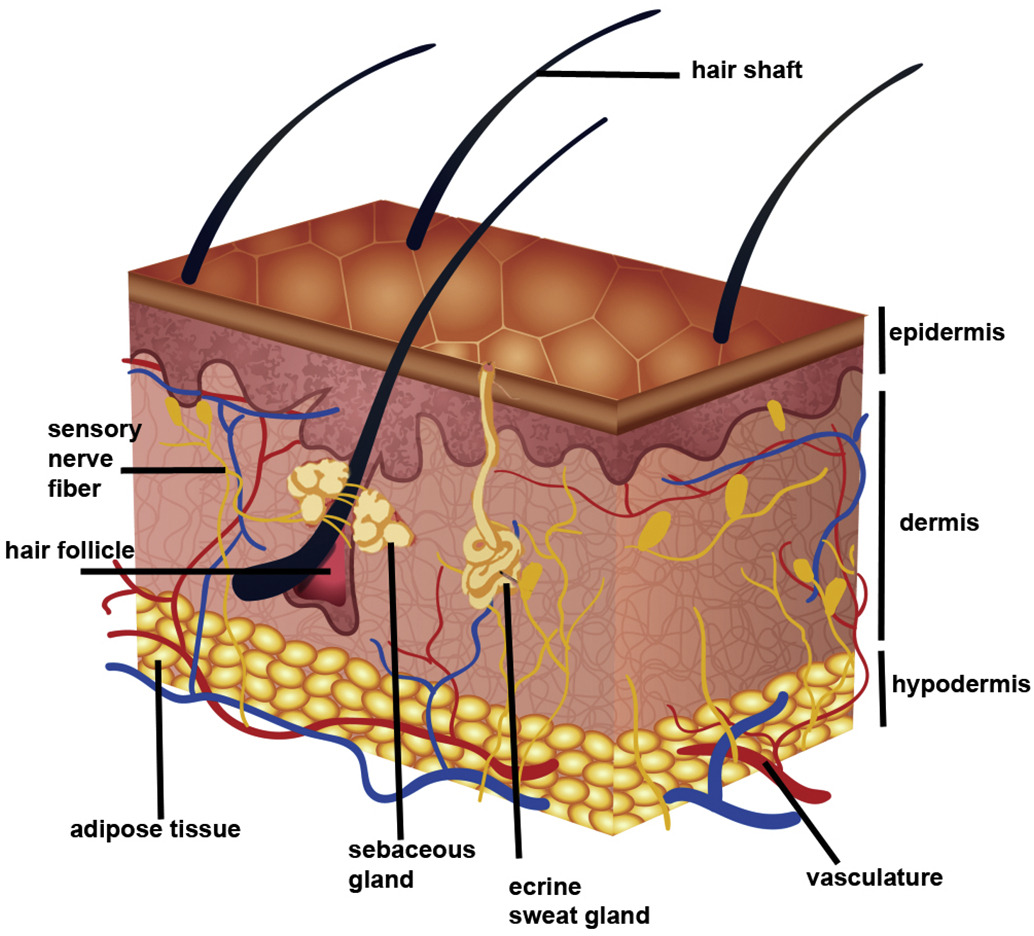
\includegraphics[width=80mm, scale = 0.5]{Figuras/skin_structure1.jpg}
    \centering
    \caption{Ilustración de las capas de la piel y sus apéndices \citep{skin_1}.}
    \label{fig:skin1_jpg}
\end{figure}

\coltext{Traducir a español y remover etiquetas no relevantes.}

Sin embargo, debido a la exposición continua a las radiaciones de la luz es común desarrollar enfermedades en la piel que afectan la forma en que las células de la piel se reproducen, causando graves daños en el tejido celular y en algunos casos resultando letal. Estas anomalías en la piel se denominan como \emph{cáncer de piel}, y se clasifican de la siguiente forma: cáncer de células basales, cáncer de células escamosas y melanomas \citep{cancer_org}.

\begin{figure}[h!]
    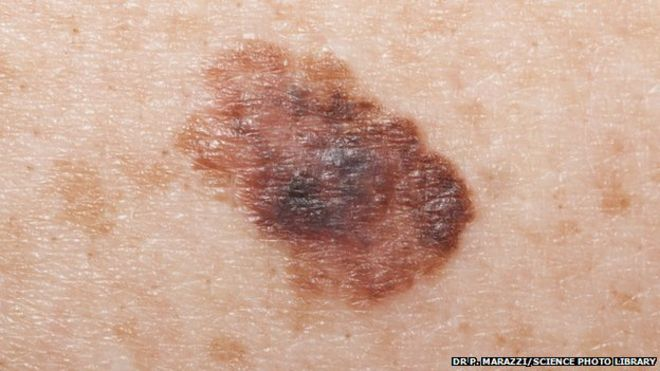
\includegraphics[width=80mm]{Figuras/skin_cancer_bbc.jpg}
    \centering
    \caption{Ejemplo de melanoma \citep{cancer_img_1}.}
    \label{fig:can_jpg}
\end{figure}

 Su detección temprana es imprescindible para reducir las probabilidades de fallecimiento. Por lo tanto es necesario seguir desarrollando tecnologías que faciliten la detección de este tipo de padecimientos de forma rápida y sencilla que vaya enfocada en aumentar la accesibilidad a dichos diagnósticos y de esta forma reducir la tasa de mortalidad por este padecimiento.

En los últimos años se han logrado muchos avances en cuanto al desarrollo de software inteligente lo cuál ha permitido un mayor acceso a diferentes servicios, una de las tecnologías que han adquirido mayor importancia es la \emph{\gls{rn}}, se trata de una tecnología que tiene la capacidad de \emph{aprender} mediante el úso de datos históricos y mediante funciones de optimización crear un modelo matemático capaz de predecir, clasificar o recrear datos futuros o desconocidos. Algunos de los sectores que han comenzado a adoptar esta tecnología son: el sector automotriz (piloto automático), el sector de manufactura (optimización de procesos), el sector de entretenimiento (recomendaciones personalizadas), el sector médico (diagnóstico de imágenes). 


\section{Hipótesis}
Es posible clasificar los píxeles en distintas categorías dentro de una imagen gracias a las avances actuales de inteligencia artificial y la técnica de segmentación. Mediante la técnica de \emph{\gls{seg}} es posible crear un reconocedor visual que no solo detecte la presencia y ubicación del elemento a reconocer, sino que, también obtenga otros datos descriptivos del elemento como el tamaño, forma y región que abarca dentro de la imagen.

\section{Objetivos}
Primero en \emph{objetivo general} se habla de manera conceptual la problemática a resolver tales como cuales son las situaciones en las que podemos optimizar la resolución de un problema mediante el uso de la red neuronal, posteriormente en los \emph{objetivos específicos} se describe de forma puntual los pasos a realizar en el presente trabajo de tésis para llegar al resultado deseado.

El \emph{objetivo general} de este trabajo de tésis es la creación de una aplicación capaz de detectar anomalías en la superficie piel que correspondan a alguno de los tipos de \emph{cáncer de piel} mediante imágenes (basalioma, carcinoma, melanoma), con el uso de la red neuronal de \emph{\gls{seg}} usando como base la arquitectura de red neuronal mencionada en \citet{wu2019fastfcn}. 


El \emph{objetivo específico}, es el implementar un modelo de red neuronal cuya entrada sean imágenes que pueden o no contener la presencia de alguno de los tipos de cáncer de piel comunes, y como salida del modelo se obtenga un mapa de características donde de haber presencia de el cáncer este se distinga mediante una región colorada en el espacio que abarca. El modelo debe cumplir con las siguientes características:

\begin{itemize}
    \item El modelo debe ser capaz de trabajar con imágenes a color o en blanco y negro.
    \item El modelo debe contar con una función capaz de evaluar la precisión.
    \item El modelo debe contar con un algoritmo capaz de optimizar la precisión.
    \item El modelo debe ser capaz de segmentar correctamente imágenes no usadas en los datos de entrenamiento.
\end{itemize}

\begin{figure}[!htp]
    \centering
    \subfloat[]{\label{a}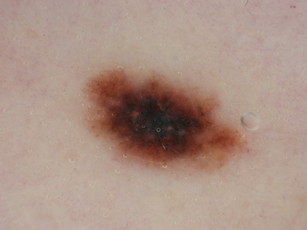
\includegraphics[width=50mm]{Figuras/input_1.png}}
    \qquad
    \subfloat[]{\label{b}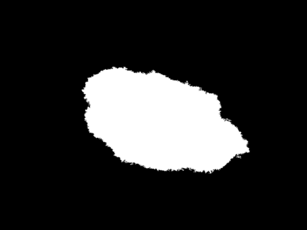
\includegraphics[width=50mm]{Figuras/mask_1.png}}
    \caption{Comparación de dato de entrada (a) y la salida deseada (b).}
    \label{data_1}
\end{figure}

En la figura \ref{data_1} (a) se observa como la imagen entrante presenta un caso de melanoma y posteriormente, en la figura \ref{data_1}(b) se puede observar la misma imagen después de pasar por una secuencia de transformaciones, esto se denomina \emph{segmentación semántica} y se refiere a la acción de separar y clasificar en una o mas categorías los objetos detectables en una imágen.

\section{Estructura de la Tesis}
En esta sección se dará una breve descripción sobre el orden en el que se desarrollan los temas y el contenido de estos.

En el capítulo 2 se habla sobre los antecedentes relacionados al presente trabajo de tesis, primero se empieza definiendo la naturaleza del problema con el que se pretende tratar, después algúnos conceptos clave que serán necesarios para la comprensión de la implementación propuesta tales como las dimensiones de los datos y los algoritmos de evaluación y optimización. 

En el capítulo 3 se habla se recopilan trabajos relacionados al método o problemática en cuestión, se estudian las características de dichos trabajos y se busca un punto de convergencia entre estos y el presente trabajo de tésis con el fin de comparar las áreas de oportunidad.

En el capitulo 4 se describe de forma estadística los datos que serán utilizados para realizar el experimento, tomando en cuenta la distribución de los pixeles en distintas regiones de la imagen, entre otros parámetros. 

En el capítulo 5 se detalla el proceso de implementación, primero se describirán las características del hardware, se describe la arquitectura del modelo y las transformaciones por las que pasará la imagen y luego se hará una comparativa con distintos modelos de redes neuronales para comparar tiempo de entrenamiento, precisión y resultado.

Finalmente, en el capítulo 6 se exponen los resultados obtenidos de la implementación del producto científico en el capítulo anterior, así como un análisis y conclusión final sobre los valores obtenidos en precision y tiempo de entrenamiento. 

\chapter{Antecedentes}
En este capítulo se introducen de forma teórica los conceptos relacionados a los tipos de cáncer y las redes neuronales, primero se define que es el \emph{cáncer de piel}, cuales son los factores que influyen en el desarollo de este padecimiento, los tipos de cáncer y las diferencias entre estos. Después algunos conceptos relacionados con las redes neuronales necesarios para un entendimiento sólido del \emph{aprendizaje profundo}, tales como los elementos clave que conforman a la red neuronal, la manera en la que esta evalúa su precisión, y el algoritmo de optimización.

\section{Cáncer de Piel}
El \emph{cáncer de piel} es una enfermedad que suele relacionarse con la aparición de lunares o manchas que no se encontraban previamente, se pueden manifestar como manchas oscuras o rojizas, bultos y/o escamas en la superficie de la piel y afecta a todos los tonos de la piel por igual. Esta enfermedad se desarrolla principalmente en partes del cuerpo expuestas al sol, sin embargo también se puede desarrollar en partes que no suelen exponerse. Algunos factores como la exposición a los rayos ultravioletas (UV), el uso de sustancias como el tabaco o el envejecimiento son factores correlacionados con la aparición del \emph{cáncer de piel}, existen dos factores de envejecimiento y se dividen en dos grupos: 

\begin{itemize}
    \item Factores intrínsecos 
    \item Factores extrínsecos 
\end{itemize}

Los factores \emph{intrínsecos} son aquellos que suceden de forma interna en la piel, un ejemplo de esto es el envejecimiento cronológico, el cual es un proceso natural que consiste en degradación del colágeno, la elastina y el adelgazamiento de la epidermis debido al envejecimiento celular al paso de los años y de el efecto de algunas hormonas.

Los factores \emph{extrínsecos} son aquellos que suceden de forma agena al organismo, como es el caso del \emph{foto-envejecimiento} el cual sucede cuando nos encontramos expuestos a los rayos ultravioletas (UV). Este factor de envejecimiento genera lesiones en las cadenas de ácido desoxirribonucleico (ADN) debido a la oxidación y afecta la regeneración de celulas, al sistema inmune y a la forma en la que se regula la pigmentación \citep{skin_aging}.

\subsection{Tipos de Cáncer de Piel}
Existe una gran variedad de tipos de \emph{cáncer de piel}, sin embargo son cuatro tipos los que destacan por tener una mayor incidencia:

\begin{itemize}
    \item melanoma
    \item cáncer de piel no melanoma
    \item carcinóma de células basales
    \item carcinóma epidermoide de piel
\end{itemize}

\coltext{Necesito mas referencias sobre esta información}

\section{Redes Neuronales}

Hasta hace algunos años, el desarollo de aplicaciones de software solía realizarse de una forma robústa, por ejemplo, si deseáramos desarrollar una aplicación de reconocimiento de imágenes de la forma tradicional sería necesario un grupo de expertos en dicho rubro, sin embargo mediante las redes neuronales es posible resolver los mismos problemas de una forma distinta mediante el uso de bases de datos. Algunos de los puntos clave que conforman una red neuronal son los siguientes:

\begin{itemize}
    \item Datos: Se debe determinar la naturaleza y la dimensión de los datos que entrarán al modelo.
    \item Modelo: Se debe crear un sistema que transforme los datos de entrada, en la salida deseada.
    \item Evaluación: El modelo debe tener la capacidad de evaluar su precisión.
    \item Optimización: El modelo debe contar con un algoritmo que optimice la precisión.
\end{itemize}

\subsection{Imágenes como Datos}
Las imágenes se pueden definir como una matriz de $m \times n \times 1$ pixeles en el caso de las imágenes de un solo canal (blanco y negro) y en el caso de imágenes a color es de $m \times n \times k$, donde $k$ es igual al numero de canales de color que tenga la imagen, siendo tres en el caso de imágenes \emph{rgb}, es importante definir si las imágenes ingresarán al modelo a color o en blanco y negro debido a que esto define el numero de nodos de entrada de este, ya que para cada pixel debe corresponder un nodo de entrada y en el caso de imágenes a color también deberá tener un número de capas de nodos de entrada igual al número de canales que tenga la imagen.

\begin{figure}[h!]
    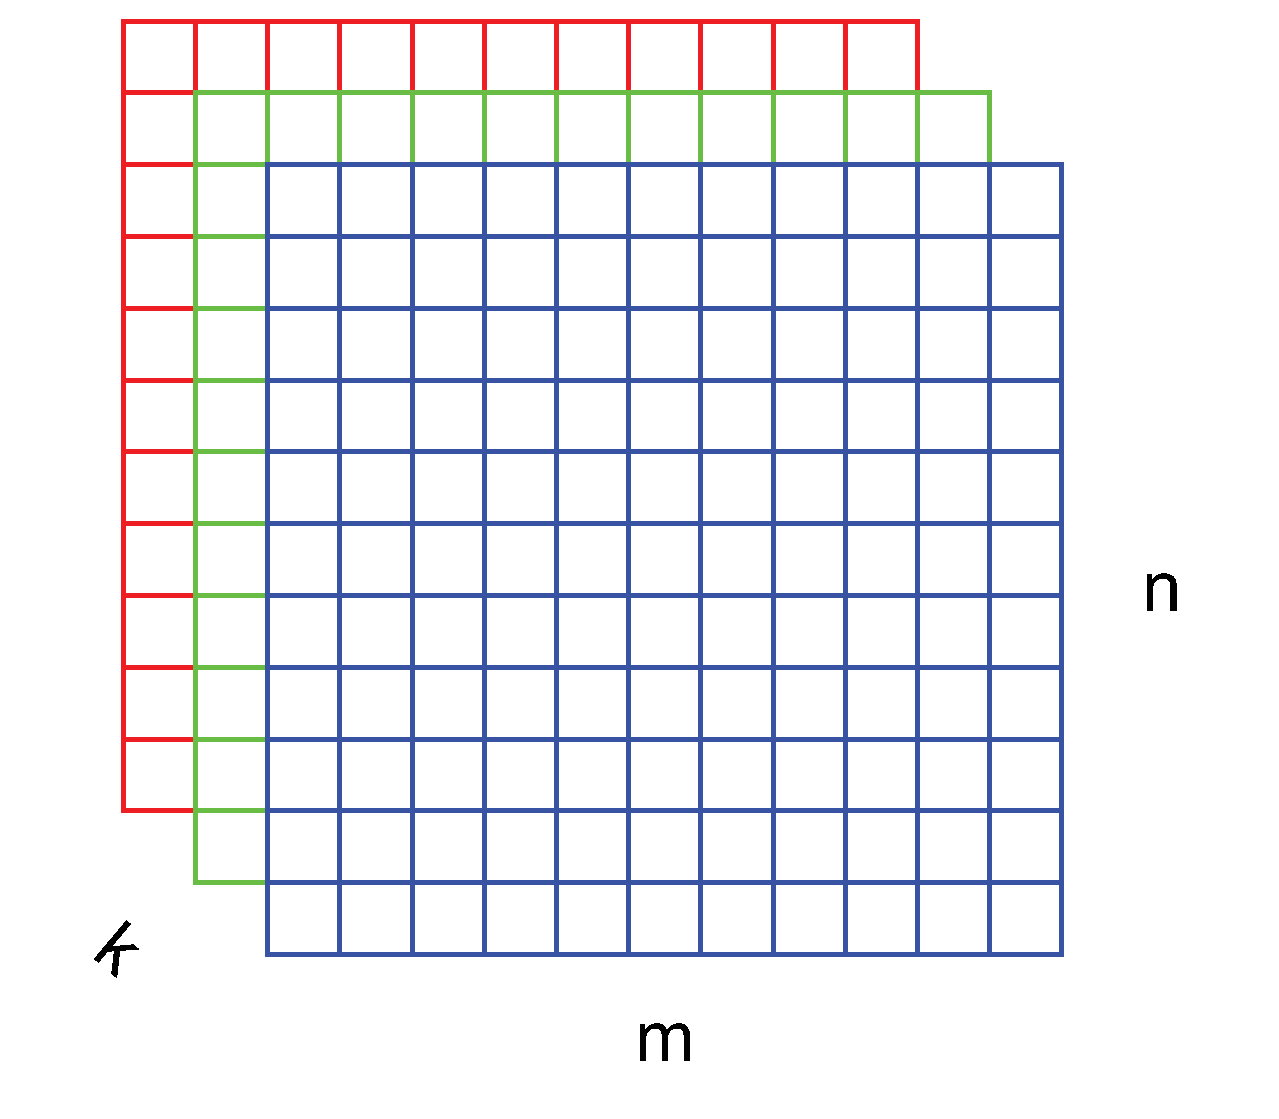
\includegraphics[width=50mm]{Figuras/rgb_matrix_2.eps}
    \centering
    \caption{Representación de las dimensiones en una imagen con tres canales de color.}
    \label{fig:rgb_mat}
\end{figure}

\coltext{Agregar representación de imagen de un canal en un subplot.}

\subsection{Modelo}
Un \emph{modelo} se puede definir como el bloque intermedio entre los datos de entrada (\emph{input}) y los datos de salida (\emph{output}), es el sistema encargado de transformar los datos de entrada en la salida deseada y consta de los siguientes componentes:

La unidad principal que compone el modelo de la red neuronal es el perceptrón, denominado \emph{nodo} en esta literatura. Se trata de una analogía matemática basada en el comportamiento de la neurona biológica, el nodo recibe $n$ entradas, las cuales son multiplicadas por el peso $p$, se suma el producto de las entradas por sus pesos $ e \times p$ y finalmente se multiplica por la funcion de activación $\phi$. 

\begin{figure}[h!]
    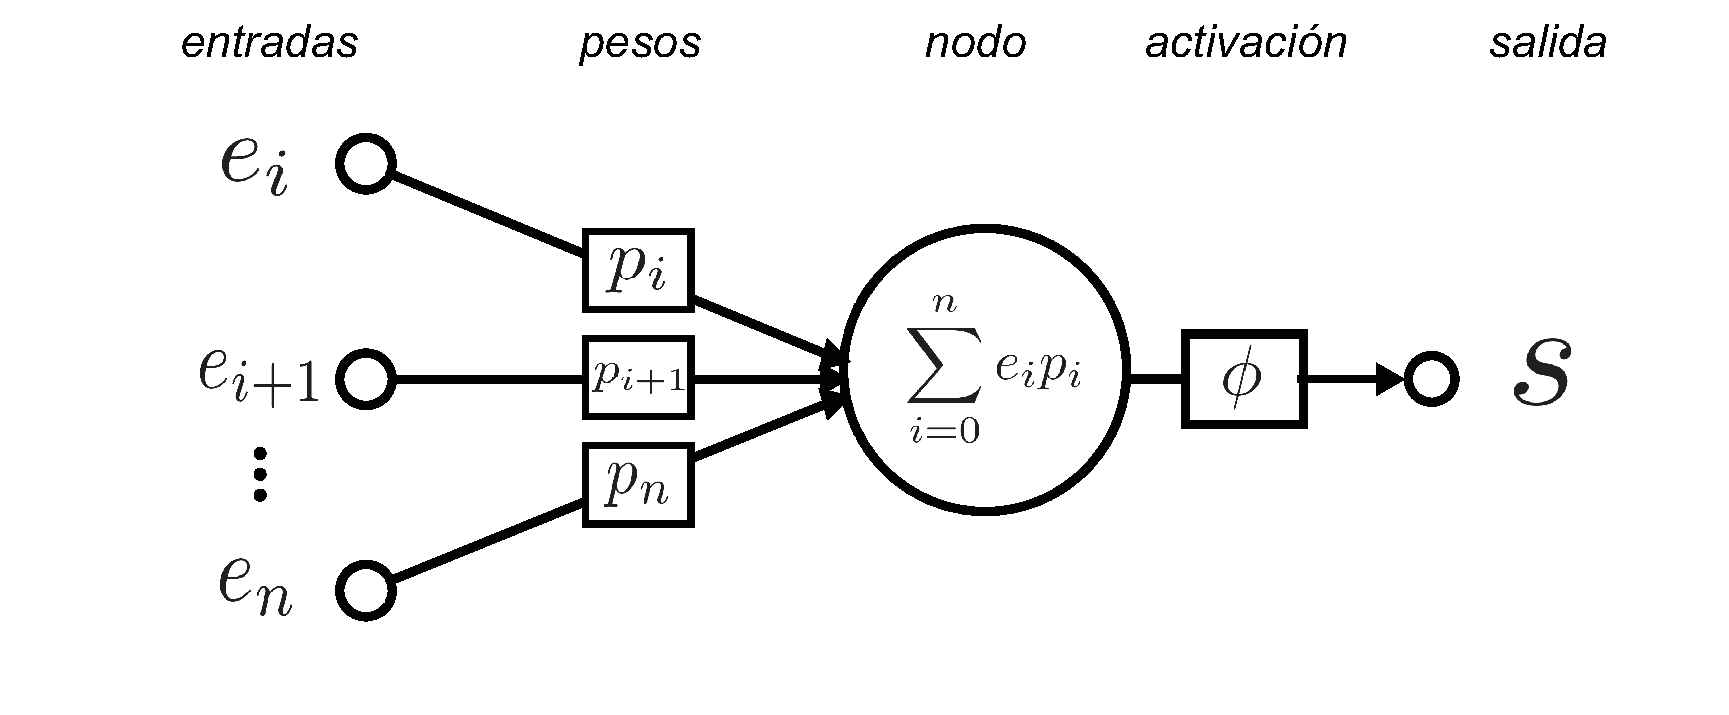
\includegraphics[width=100mm]{Figuras/neural_network.eps}
    \centering
    \caption{Ejemplo de un perceptrón.}
    \label{fig:percep}
\end{figure}

Partiendo de lo anterior, creando arreglos con estos nodos podemos formar estructuras denominadas \emph{redes neuronales}, las cuales cuentan con las siguientes características para cumplir las funciones básicas de clasificación:

\begin{itemize}
    \item Capa de nodos de entrada (\emph{input nodes}): Se trata de la primera capa del modelo, en el caso de imágenes a cada pixel le corresponde un nodo de entrada. Estos nodos deben tener las mismas dimensiones que las imágenes de entrada.
    \item Capa de nodos ocultos (\emph{hidden nodes}): Las dimensiones de estos nodos pueden ser diferentes a los de entrada y tener varias capas ocultas, sin embargo esto puede afectar la complejidad y precisión del modelo.
    \item Capa de nodos de salida (\emph{output nodes}): Esta es la capa de salida del modelo, las dimensiones de la capa de salida determinan las dimensiones del dato resultante.
    \item Función de activación (\emph{activation}): Se trata de una función dentro de cada nodo que interactúa con el valor entrante y se multiplica por el peso.
    \item Pesos (\emph{weights}): Se trata de un valor entre el nodo de la capa actual y el nodo siguiente inicializado de forma aleatoria y después ajustado por un algoritmo para aproximar la salida al valor real.
    \item Bías (\emph{bias}): Se trata de un valor constante que se suma al resultado de la función de activación y el peso, de esta forma se puede ajustar que tan fácil o difícil es activar un nodo.
\end{itemize}


\subsection{Evaluación y Optimización}
Para realizar el proceso de \emph{aprendizaje} del modelo, primero se debe evaluar cuál es el estado actual de las predicciones. Para esto es necesario evaluar que distancia existe entre el valor predicho y el valor real, esto se puede lograr mediante una \emph{función de pérdida} que se encargue de determinar que tanta diferencia(\emph{loss}) existe en las estimaciones del modelo con los pesos actuales.

Un ejemplo de la función de pérdida es el de la función logarítmica del costo (\emph{log-likelihood}), como se muestra a continuación en donde:

$l(\mathbf{y}, \hat{\mathbf{y}}) = - \sum_{j=1}^q y_j \log \hat{y}_j$ 

\begin{itemize}
    \item $q$, representa el número de clases entre las debe cuales predecir.
    \item $y_j$, representa valor real.
    \item $\hat{y_j}$, representa valor estimado por el modelo.
    \item $j$, representa la posición en el indizado de las clases.
\end{itemize}

Ya que se tiene calculada la pérdida del modelo en su configuración actual, es necesario actualizar el valor de todos los pesos dentro del modelo para poder acercarnos al valor real. Aquí es donde se requiere un algoritmo que primero determine si el peso de cada nodo debe aumentar o disminuir, y después de determinar la dirección realizar un ajuste antes de volver a evaluar el modelo.

Para esto existe el algoritmo de \emph{gradiente descendiente}, comienza en un punto inicial y repetidamente da un paso hacia la dirección opuesta del gradiente en cada punto y así minimizar el \emph{costo}. A continuación se representa la forma del algoritmo:

\coltext{Utilizar environment de pseudocódigo.}
\begin{tabbing}
    \hspace*{1.5in} \= \hspace*{0.7in} \= \hspace*{.25in} \= \hspace*{.25in} \= \hspace*{.25in} \=\kill
    \>{\bf Para} $k=0,1,2 \dots n$ {\bf Realiza } \\
    \>\> $g_k \leftarrow \nabla f(x_k)$ \\
    \>\> $x_{k+1} \leftarrow x_k - t_k g_k$ \\
    \>{\bf Fin} \\
\end{tabbing}

\chapter{Estado del Arte}
En este capítulo se estudian las literaturas relacionadas con el presente trabajo de tesis con el objetivo de hacer una comparativa entre distintos métodos para resolver el mismo problema, o implementaciones similares para resolver problemas distintos.

En la primera sección \emph{trabajos similares} se recopilan trabajos con características relacionadas al presente trabajo de tesis, ya sea relacionados con el método o con el problema que se pretende resolver, se describirá el tema que abarcan y los puntos que lo relacionan con el trabajo aquí presente. 

En la segunda sección \emph{análisis comparativo} se comparan las distintas características de los trabajos revisados, de esta forma podemos determinar las principales diferencias así como las ventajas y desventajas de cada trabajo. Así mismo se recopilaran todas estas diferencias en una tabla para visualizar mejor estas características.

Finalmente en las \emph{áreas de oportunidad} se realiza una conclusión acerca de los resultados en la tabla comparativa.

\section{Trabajos Similares}

A continuación se mencionan los trabajos revisados en los que se puede obtener un punto de convergencia ya sea en los métodos similares utilizados para resolver problemas diferentes o en su defecto métodos distintos para resolver problemas similares.

\citet{DBLP:journals/corr/BadrinarayananK15}, en este trabajo se habla sobre la arquitectura denominada \emph{SegNet} utilizada principalmente para la conducción autónoma y la detección de peatones, se describe como una arquitectura convolucional, con la característica de que es una jerarquía de codificador-decodificador donde a cada codificación (\emph{encoding}) corresponde una capa de agrupación de máximos (\emph{max pooling}) y un decodificador. Inspirado principalmente en la arquitectura \emph{VGG16}, con la diferencia de que el componente clave en esta arquitectura es el uso de convoluciones en lugar de la capa completamente conectada de nodos (\emph{fully-connected-layer}) a la salida.

\citet{DBLP:journals/corr/RonnebergerFB15}, propone uno de los primeros modelos de la redes neuronales convolucionales denominada \emph{U-net} dirigida al análisis de imágenes del area médica. Este trabajo consiste en una arquitectura con dos trayectorias: la trayectoria de contracción de la imagén y la trayectoria de expansión. En la trayectoria de contracción de la imagen se aplica una secuencia de convoluciones de dimension $3 \times 3$ con solapado, seguido de una función de activación de rectificación linear unitaria (\emph{ReLu}) y posteriormente una operación de agrupación de máximos (\emph{max pooling}) para la compresión de la imagen (\emph{downsampling}). Por otro lado, la trayectoria de expansión consiste de el escalado de la imagen (\emph{upsampling}), en cada paso se aplica una capa de convolución de $2 \times 2$ a la cuál se concatena una imagen recortada del mapa de características de la trayectoria de contracción y dos convoluciones de $3 \times 3$ seguidos de una activación ReLu cada una. En total la arquitectura tiene 23 convoluciones (U-net) .

\citet{DBLP:journals/corr/ChenPK0Y16}, en este trabajo se habla de la arquitectura denominada \emph{Deep Lab}, la cual propone un acercamiento distinto a la parte de la reconstrucción en las capas finales del modelo. Al igual que otras arquitecturas cuenta con capas de convolución. agrupación de máximos y activación de rectificación linear unitaria, sin embargo, el componente clave aquí es la denominada convolución de hoyos (\emph{atrous convolution}), la cual es una modificación al filtro de convolución basado en la transformada de wavelet para el escalado del mapa de características (\emph{upsampling}). De esta forma se obtiene una alternativa al uso de capas de deconvolución y así se aumenta la resolución del mapa de características a la salida del modelo sin aumentar el tiempo de computación o la cantidad de parametros.

\citet{DBLP:journals/corr/TeichmannWZCU16}, nos habla sobre la reducción de computaciones en en los modelos de redes neuronales convolucionales mediante la unificación de las tres tareas principales de estas: clasificación, detección y segmentación. Denominada como multi-red neuronal (\emph{multinet}) se trata de una arquitectura tipo codificador-decodificador en donde el decodificador esta compuesto de tres ramas las cuales corresponden a las tareas de clasificación, detección y segmentación por lo que se realizan las tres tareas de forma simultanea partiendo de la misma entrada (\emph{multi-tasking}) y usando la salida de cada una de las ramas para el ajuste fino de los parametros del modelo (\emph{fine-tuning}).  

\citet{KRONER2020261}, habla sobre un módelo de codificación-decodificación contextual basado en el proceso en el que los humanos obtenemos la información espacial de los escenarios visuales complejos, mediante un mapa topográfico de las salientes. Se basa en más en el proceso biológico con el que se obtiene la información espacial que en los métodos matemáticos para calcularla, dicho lo anterior, los principales componentes para determinar una saliente son color, la intensidad y la orientación.  

\citet{KADAMPUR2020100282}, proponen el úso de los servicios de nube en conjunto con las redes neuronales profundas y el diseño de modelos utilizando modelos pre-entrenados. Para esto utilizan la herramienta de \emph{deep learning studio (DLS)}, la cual es un software que permite el uso de tarjetas gráficas (\emph{GPU}) localizadas en la nube o localmente, y también permite el uso de múltiples tarjetas de forma simultanea (\emph{multi-GPU}), la arquitectura usada para la detección de cáncer de piel en este trabajo es de una red neuronal profunda de clasificación, por lo que el modelo se codifica mediante convoluciones y se decodifica mediante capas de aplanamiento (\emph{flatten layer}) para posteriormente entrar a una capa de nodos completamente conectada (\emph{fully-connected-layer}) y obtener dos posibles resultados: es cáncer o no es cáncer.

\citet{zhou2019emerging} 

\citet{DBLP:journals/corr/LucCCV16}

\citet{JAIN2015735}

\section{Analisis Comparativo}
A continuación se evalúan las características que poseen los distintos trabajos mencionados en la sección anterior, para esto se deberá definir una serie de características a evaluar que sirvan como punto de referencia entre estos trabajos, dichas características son las siguientes:

\begin{itemize}
    \item Modelo. Tipo de arquitectura del modelo.
    \item Clasificación. El sistema puede clasisificar entre distintas categorías.
    \item Segmentación. El sistema puede segmentar las imagenes.
    \item Supervisado. El sistema requiere de datos de entrenamiento.
    \item Pre-entrenamiento. El sistema requiere de pesos pre-entrenados.
    \item Evaluación. Método que el sistema utiliza para determinar su presición.
    \item Optimización. Algoritmo que el sistema utiliza para mejorar su precisión.
\end{itemize}

\begin{table}[hbt!]
    \caption{Similitudes y diferencias entre los trabajos revisados.}
    \begin{adjustbox}{width=\textwidth}
        \begin{tabular}{|c|c|c|c|c|c|c|c|}
            \hline
            Trabajo & Modelo & Clasificación & Segmentación & Supervisado & Pre-entrenamiento & Evaluación & Optimización\\
            \hline
            \citet{DBLP:journals/corr/BadrinarayananK15} & FCN & \cmark & \cmark & \cmark & \cmark & Log-likelihood & SGD\\
            \hline
            \citet{DBLP:journals/corr/RonnebergerFB15} & U-net & \cmark & \cmark & \cmark & \cmark & Log-likelihood & SGD\\
            \hline
            \citet{DBLP:journals/corr/ChenPK0Y16} & DeepLab & \cmark & \cmark & \cmark & \cmark & G & H\\
            \hline
            \citet{DBLP:journals/corr/TeichmannWZCU16} & MultiNet & \cmark & \cmark & \cmark & \cmark & G & H\\
            \hline
            \citet{KRONER2020261} & VGG16 & \cmark & \cmark & \cmark & \cmark & G & H\\
            \hline
            \citet{KADAMPUR2020100282} & CNN & \cmark & \xmark & \cmark & \xmark & G & H\\
            \hline
            \citet{zhou2019emerging} & NN & \cmark & \cmark & \cmark & \cmark & G & H \\
            \hline
            \citet{DBLP:journals/corr/LucCCV16} & ANN & \cmark & \cmark & \cmark & \cmark & G & H\\
            \hline
            \citet{JAIN2015735} & A.B.C.D & \cmark & \xmark & \xmark & \xmark & G & H\\
            \hline
            \rowcolor{Green}
            \citet{wu2019fastfcn} & FastFCN & \cmark & \cmark & \cmark & \cmark & G & H\\
            \hline
        \end{tabular}
    \end{adjustbox}
    \end{table}

\section{Áreas de Oportunidad}
En esta sección se señalan las características de los trabajos mencionados en la sección anterior y se compara con las características del método propuesto en este trabajo de tesis para obtener una comparativa sobre las áreas de oportunidad.

\chapter{Implementación de la Solución}

\chapter{Resultados}

\chapter{Conclusiones}
